\documentclass[a4paper,12pt]{article}
\usepackage{a4wide,amssymb,epsfig,latexsym,multicol,array,hhline,fancyhdr}
\usepackage{vntex}
\usepackage{amsmath}
\usepackage{lastpage}
\usepackage[lined,boxed,commentsnumbered]{algorithm2e}
\usepackage{enumerate}
\usepackage{listings}
\usepackage{xcolor}
\usepackage{graphicx}
\usepackage{array}
\usepackage{tabularx, caption, booktabs}
\usepackage{multirow}
\usepackage{multicol}
\usepackage{rotating}
\usepackage{graphics}
\usepackage{geometry}
\usepackage{footnote}
\usepackage{setspace}
\usepackage{tikz}
\usepackage{xfrac}
\usepackage{indentfirst}
\usetikzlibrary{shapes, arrows, arrows.meta, positioning, fit, calc, snakes, backgrounds}
\usepackage{bm}
\usepackage{float}
\usepackage{subcaption}
\usepackage[colorlinks]{hyperref}
\usepackage[
 sort=none,
 abbreviations,
 symbols,
 stylemods,style=list,
 nogroupskip, nonumberlist, nomain
]{glossaries-extra}

% Colors
\definecolor{codegray}{rgb}{0.5,0.5,0.5}
\definecolor{codepurple}{rgb}{0.6,0.2,0.6}
\definecolor{backcolor}{rgb}{0.95,0.95,0.95}
\definecolor{mathblue}{RGB}{0,114,188}
\definecolor{bwBlack}{HTML}{000000}
\definecolor{bwGray}{HTML}{555555}
\definecolor{bwOffWhite}{HTML}{F7F7F7}
\def\labelitemi{--}

% Code style
\lstdefinestyle{custom}{
    backgroundcolor=\color{backcolor},
    commentstyle=\color{codegray},
    keywordstyle=\color{blue},
    stringstyle=\color{codepurple},
    basicstyle=\ttfamily\small,
    breakatwhitespace=false,
    breaklines=true,
    captionpos=b,
    keepspaces=true,
    numbers=left,
    numberstyle=\tiny\color{codegray},
    rulecolor=\color{black},
    showspaces=false,
    showstringspaces=false,
    showtabs=false,
    tabsize=2
}
\lstset{style=custom}

% Formatting
\DeclareMathOperator{\arccot}{arccot}
\captionsetup[table]{name=Bảng}
\captionsetup[figure]{name=Hình}
\newenvironment{Description}{\list{}{%
    \let\makelabel\descriptionlabel
    \setlength{\rightmargin}{\leftmargin}
    \setlength{\labelwidth}{0pt}
    }}{\endlist}

\hypersetup{urlcolor=blue,linkcolor=black,citecolor=black,colorlinks=true}

% TikZ Styles for Neural Network & Pipeline Diagrams
\tikzset{
  tok/.style={
    rectangle, draw=bwGray, line width=0.5pt, fill=bwOffWhite,
    rounded corners=1.5pt, minimum width=0.85cm, minimum height=0.45cm,
    font=\scriptsize\ttfamily, align=center
  },
  emb/.style={
    rectangle, draw=bwBlack, line width=0.6pt, fill=white,
    minimum width=0.85cm, minimum height=0.45cm,
    font=\scriptsize, align=center
  },
  cell/.style={
    rectangle, draw=bwBlack, line width=0.7pt, fill=white,
    rounded corners=2pt, minimum width=1.15cm, minimum height=0.55cm,
    font=\scriptsize\bfseries\sffamily, align=center
  },
  cellbwd/.style={cell, fill=bwOffWhite},
  neuron/.style={
    circle, draw=bwBlack, line width=0.65pt, fill=white,
    minimum size=0.34cm, inner sep=0pt
  },
  neurondark/.style={neuron, fill=bwBlack},
  opcircle/.style={
    circle, draw=bwBlack, line width=0.65pt, fill=white,
    minimum size=0.38cm, inner sep=0pt, font=\scriptsize\bfseries
  },
  modbox/.style={
    rectangle, draw=bwBlack, line width=0.7pt, fill=white,
    rounded corners=2pt, align=center, font=\footnotesize\sffamily, inner sep=5pt
  },
  modboxfill/.style={modbox, fill=bwOffWhite},
  modboxdark/.style={modbox, fill=bwBlack, text=white},
  arr/.style={-{Stealth[length=1.8mm,width=1.2mm]}, draw=bwBlack, line width=0.65pt},
  arrgray/.style={-{Stealth[length=1.5mm,width=1.0mm]}, draw=bwGray, line width=0.55pt},
  synapse/.style={draw=bwGray, line width=0.45pt},
  dashedframe/.style={
    rectangle, draw=bwGray, dashed, line width=0.6pt,
    rounded corners=2pt, inner sep=6pt
  }
}

% Header/Footer
\setlength{\headheight}{40pt}
\pagestyle{fancy}
\fancyhead{}
\fancyhead[L]{
 \begin{tabular}{rl}
    \begin{picture}(25,15)(0,0)
    \put(0,-8){
\includegraphics[width=10mm, height=10mm]{hcmut.jpg}}
   \end{picture}&
	\begin{tabular}{l}
		\textbf{\bf \ttfamily Ho Chi Minh City University of Technology}\\
		\textbf{\bf \ttfamily Faculty of Computer Science and Engineering}
	\end{tabular}
 \end{tabular}
}
\fancyhead[R]{\begin{tabular}{l}\tiny \bf \\\tiny \bf \end{tabular}}
\fancyfoot{}
\fancyfoot[L]{\scriptsize \ttfamily Lập trình cho Khoa học Dữ liệu và Trí tuệ Nhân tạo}
\fancyfoot[R]{\scriptsize \ttfamily Trang {\thepage}/\pageref{LastPage}}
\renewcommand{\headrulewidth}{0.3pt}
\renewcommand{\footrulewidth}{0.3pt}

\setcounter{secnumdepth}{4}
\setcounter{tocdepth}{4}

\begin{document}

% =======================================================================
% TITLE PAGE
% =======================================================================
\begin{titlepage}
\begin{tikzpicture}[remember picture,overlay]
  \draw[line width=2pt]
    ($(current page.north west) + (1cm,-1cm)$) rectangle
    ($(current page.south east) + (-1cm,1cm)$);
\end{tikzpicture}
\begin{center}
{\large \textbf{ĐẠI HỌC QUỐC GIA THÀNH PHỐ HỒ CHÍ MINH}}\\[0.3cm]
    {\large \textbf{TRƯỜNG ĐẠI HỌC BÁCH KHOA}}\\[0.3cm]
    {\large \textbf{KHOA KHOA HỌC VÀ KỸ THUẬT MÁY TÍNH}}\\[1cm]
\end{center}

\vspace{0.2cm}

\begin{figure}[h!]
\begin{center}

\includegraphics[width=4cm]{hcmut.jpg}
\end{center}
\end{figure}
\vspace{0.2cm}
\begin{flushleft}
    \large \textbf{Lập trình cho Khoa học Dữ liệu và Trí tuệ Nhân tạo} \\
    \rule{\linewidth}{0.3pt} \\
    \begin{center}
        \huge \textbf{HỌC ĐA NHIỆM PHÂN LOẠI CẢM XÚC VÀ CHỦ ĐỀ PHẢN HỒI SINH VIÊN} \\
        \rule{\linewidth}{0.3pt}
    \end{center}
\end{flushleft}

\vspace{0.5cm}
\begin{center}
\renewcommand{\arraystretch}{1.45}
\setlength{\tabcolsep}{10pt}
\begin{tabular}{ll}
\textbf{Giảng viên hướng dẫn:} & ThS. Trần Huy \\
\textbf{Sinh viên thực hiện:} & Phạm Quang Hiếu -- 2310974 \\
& Nguyễn Thiên Hào -- 2310853 \\
& Nguyễn Trung Hiếu -- 2310965
\end{tabular}
\end{center}

\vfill
\begin{center}
{\footnotesize TP. HỒ CHÍ MINH, THÁNG 11 NĂM 2026}
\end{center}
\end{titlepage}

% =======================================================================
\tableofcontents
\newpage

% =======================================================================
% 1. BÀI TOÁN, MỤC TIÊU VÀ BỘ CHỈ SỐ ĐÁNH GIÁ
% =======================================================================
\section{Bài toán, Mục tiêu và Bộ chỉ số Đánh giá}

\subsection{Bối cảnh và Đặt vấn đề}
Trong môi trường giáo dục đại học, phản hồi của sinh viên cuối mỗi học kỳ là nguồn dữ liệu quan trọng giúp nhà trường đánh giá chất lượng giảng dạy, chương trình đào tạo và cơ sở vật chất. Khi số lượng khảo sát lớn, việc phân loại thủ công vừa tốn nhân lực vừa khó đảm bảo tính nhất quán.

Thay vì xây dựng hai mô hình độc lập cho hai tác vụ tách rời, bài tập lớn này áp dụng hướng tiếp cận \textbf{Học đa nhiệm (Multi-Task Learning -- MTL)} nhằm dự đoán đồng thời hai nhãn đầu ra từ cùng một câu phản hồi tiếng Việt:
\begin{itemize}
    \item \textbf{Phân loại cảm xúc (Sentiment Classification -- 2 lớp):} \texttt{negative} (tiêu cực, nhãn \texttt{0}) và \texttt{positive} (tích cực, nhãn \texttt{1}).
    \item \textbf{Phân loại chủ đề (Topic Classification -- 3 lớp):} \texttt{lecturer} (giảng viên, nhãn \texttt{0}), \texttt{training\_program} (chương trình đào tạo, nhãn \texttt{1}) và \texttt{facility} (cơ sở vật chất, nhãn \texttt{2}).
\end{itemize}

Việc dùng chung bộ mã hóa văn bản (\textit{shared text encoder}) giúp mô hình khai thác mối liên hệ ngữ nghĩa giữa thái độ đánh giá và đối tượng được nhắc tới, đồng thời giảm một nửa chi phí lưu trữ mô hình và thời gian suy luận so với hai mô hình đơn nhiệm.

\subsection{Bộ chỉ số đánh giá}
Do tập dữ liệu có sự mất cân bằng lớp ở tác vụ Topic, cả ba mô hình được đánh giá trên cùng tập kiểm thử ($N_{\text{test}} = 2{,}884$) bằng các chỉ số:
\begin{itemize}
    \item \textbf{Accuracy:} Tỷ lệ mẫu dự đoán đúng trên tổng số mẫu kiểm thử cho từng tác vụ.
    \item \textbf{Macro-F1:} Trung bình cộng F1-score của từng lớp (không trọng số), phản ánh trung thực hiệu năng trên cả lớp đa số lẫn lớp thiểu số:
    \[
        \text{Macro-F1} = \frac{1}{C} \sum_{c=1}^{C} \frac{2 \cdot \text{Precision}_c \cdot \text{Recall}_c}{\text{Precision}_c + \text{Recall}_c}
    \]
    \item \textbf{Combined Validation F1:} Trung bình cộng Macro-F1 của hai tác vụ dùng để theo dõi hội tụ và điều chỉnh learning rate trên tập validation.
\end{itemize}

% =======================================================================
% 2. KHẢO SÁT DỮ LIỆU VÀ TIỀN XỬ LÝ
% =======================================================================
\section{Khảo sát Dữ liệu và Tiền xử lý}

\subsection{Nguồn dữ liệu và Quy trình lọc nhãn}
Nghiên cứu sử dụng bộ dữ liệu phản hồi sinh viên tiếng Việt gồm ba tập tách biệt: huấn luyện (\textit{train}), kiểm định (\textit{validation}) và kiểm thử (\textit{test}). Quy trình chuẩn hóa nhãn được thực hiện như sau:
\begin{enumerate}
    \item Loại bỏ các mẫu có nhãn cảm xúc trung tính (\textit{Neutral}) và ánh xạ nhãn tích cực về dạng nhị phân (\texttt{0}: \texttt{negative}, \texttt{1}: \texttt{positive}).
    \item Loại bỏ các mẫu thuộc nhóm chủ đề khác (\textit{Others}) để tập trung vào ba chủ đề cốt lõi (\texttt{lecturer}, \texttt{training\_program}, \texttt{facility}).
\end{enumerate}

\begin{table}[H]
\centering
\caption{Thống kê số lượng mẫu trước và sau khi lọc nhãn theo từng tập dữ liệu.}
\small
\renewcommand{\arraystretch}{1.35}
\setlength{\tabcolsep}{12pt}
\begin{tabular}{lrrr}
\toprule
\textbf{Tập dữ liệu} & \textbf{Số mẫu gốc} & \textbf{Sau khi lọc} & \textbf{Tỉ lệ giữ lại (\%)} \\
\midrule
Train & 11,426 & 10,567 & 92.5\% \\
Validation & 1,583 & 1,441 & 91.0\% \\
Test & 3,166 & 2,884 & 91.1\% \\
\midrule
\textbf{Tổng cộng} & \textbf{16,175} & \textbf{14,892} & \textbf{92.1\%} \\
\bottomrule
\end{tabular}
\end{table}

\subsection{Phân tích phân bố nhãn}

\begin{figure}[H]
\centering
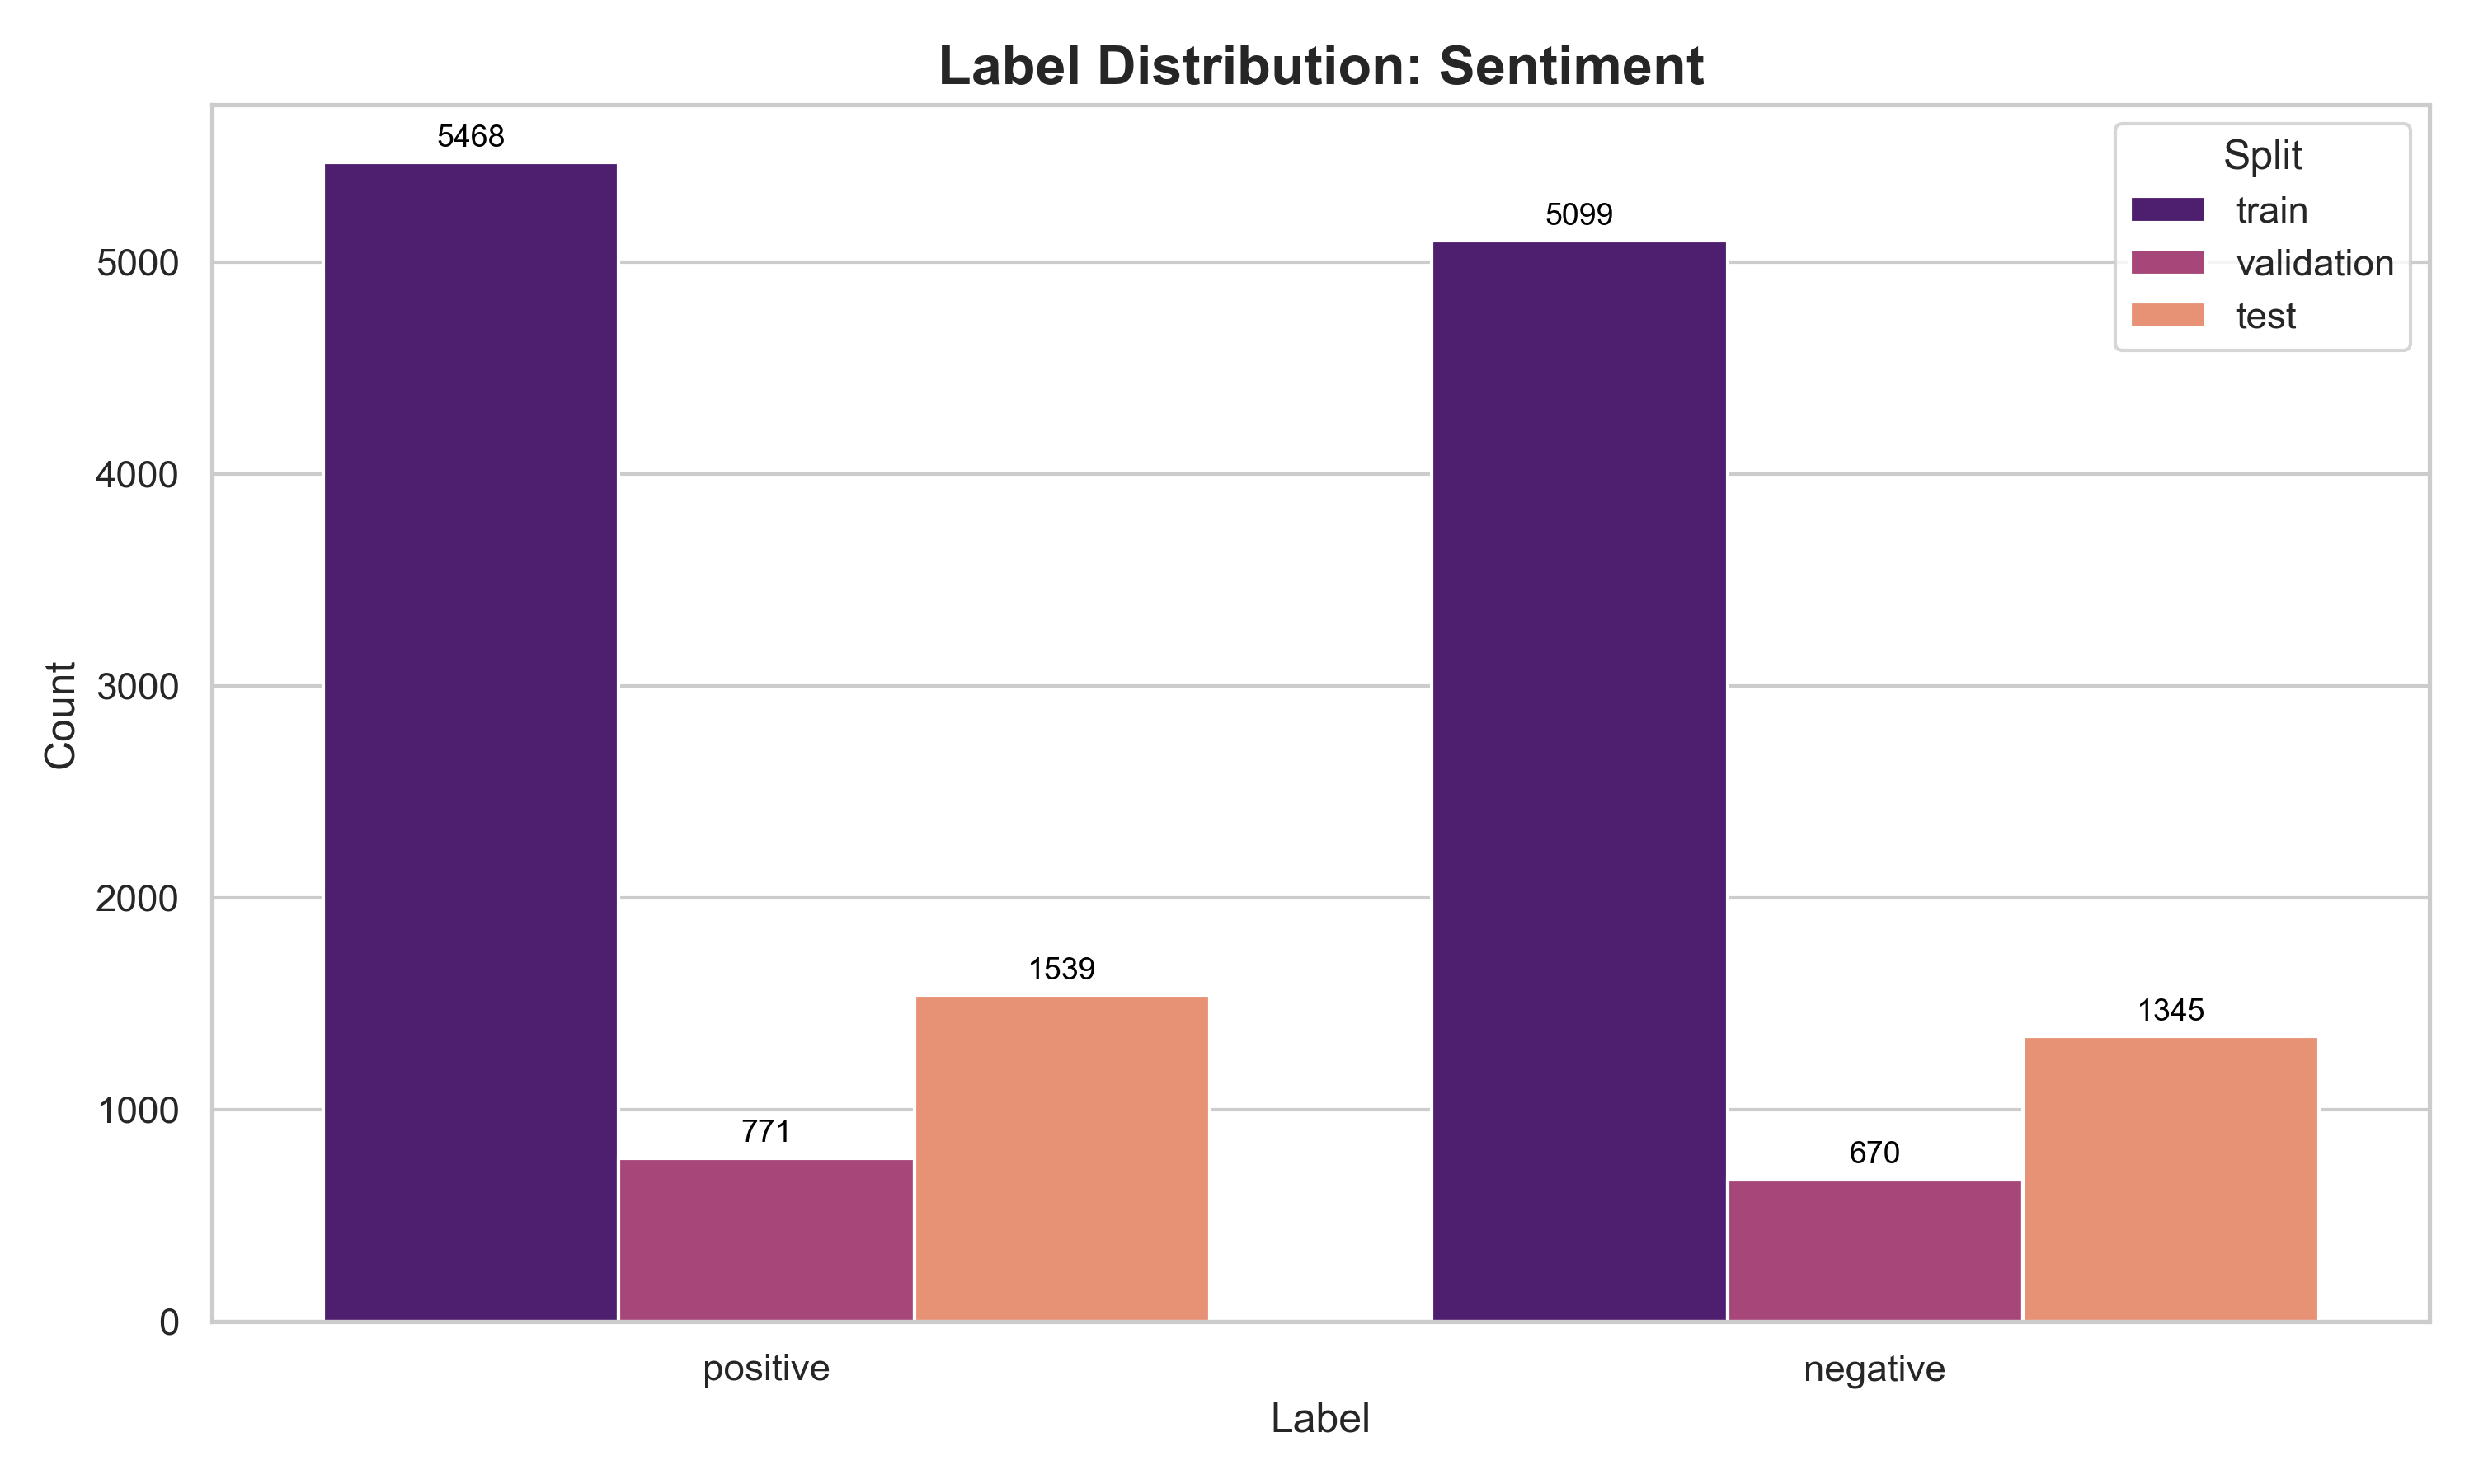
\includegraphics[width=\linewidth]{../images/sentiment_distribution.png}
\caption{Phân bố nhãn cảm xúc trên 3 tập Train, Validation và Test.}
\label{fig:sent_dist}
\end{figure}

Như thể hiện ở Hình~\ref{fig:sent_dist}, hai lớp \texttt{negative} và \texttt{positive} phân bố khá cân bằng (trên tập Test gồm 1,345 mẫu \texttt{negative} -- 46.6\% và 1,539 mẫu \texttt{positive} -- 53.4\%). Do đó hàm mất mát Cross-Entropy chuẩn kết hợp làm mịn nhãn nhẹ ($\alpha_{\text{sent}} = 0.1$) đã đủ hiệu quả mà không cần cân bằng lại trọng số lớp.

\begin{figure}[H]
\centering
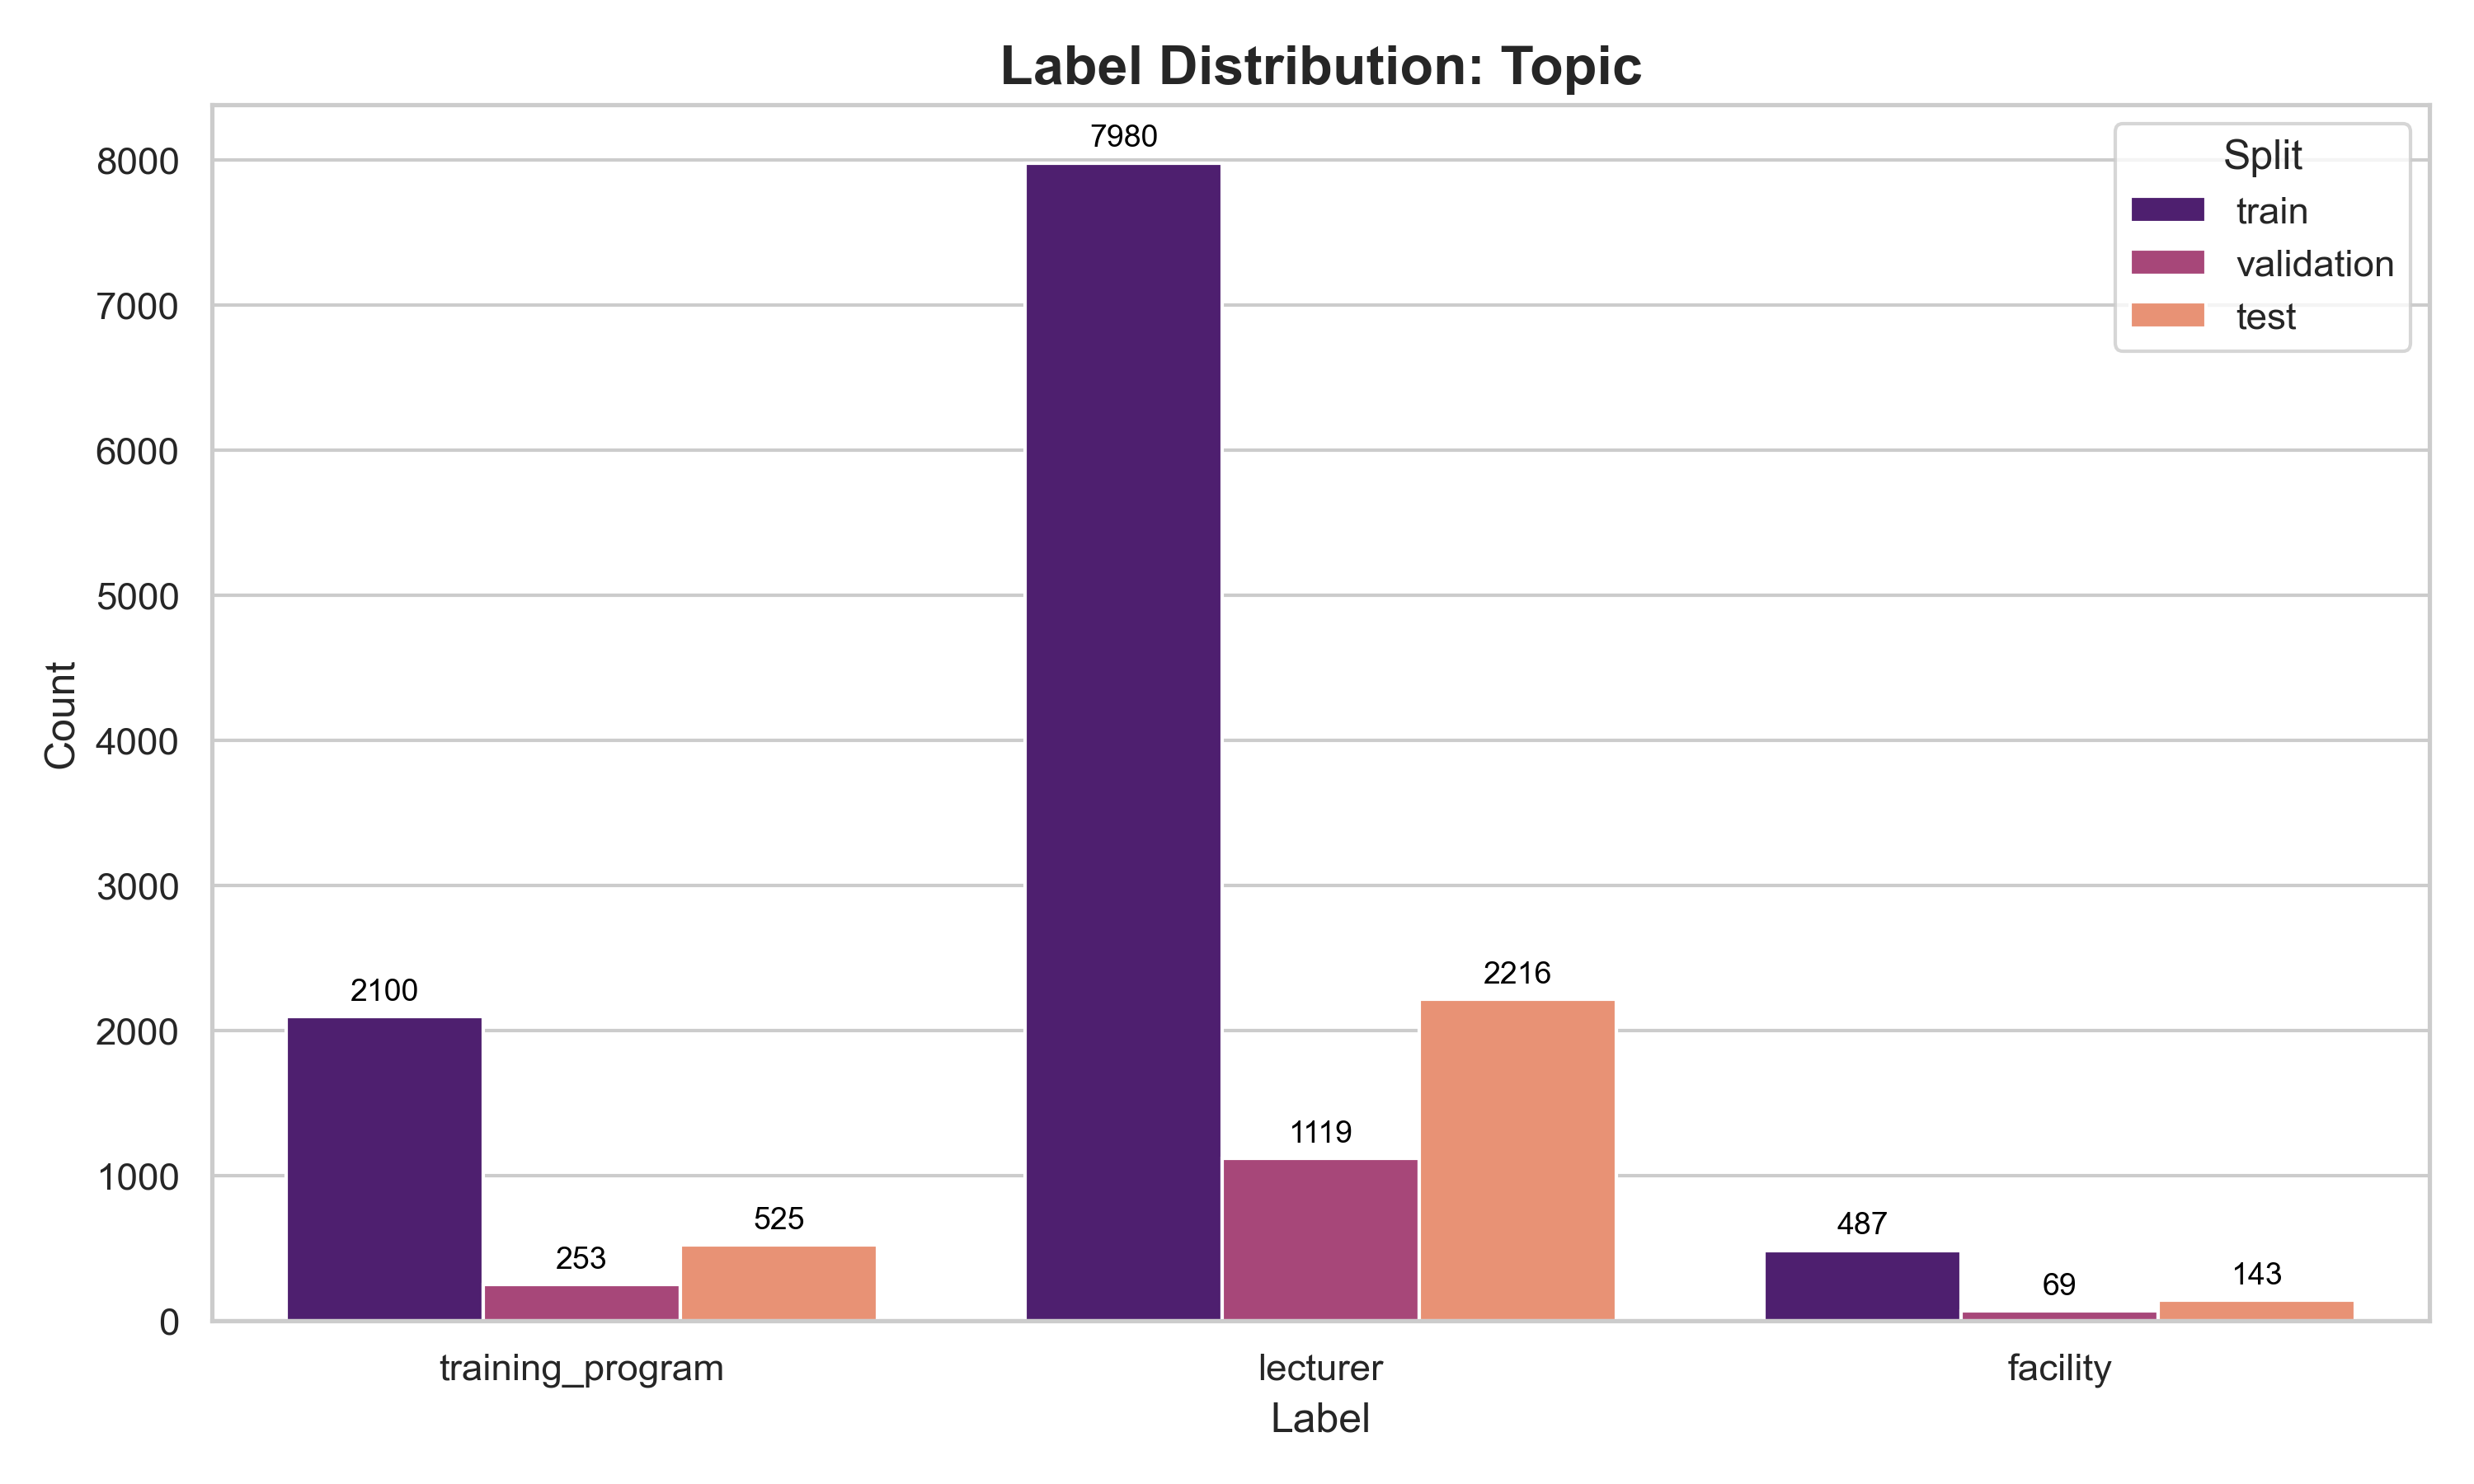
\includegraphics[width=\linewidth]{../images/topic_distribution.png}
\caption{Phân bố nhãn chủ đề trên 3 tập Train, Validation và Test.}
\label{fig:topic_dist}
\end{figure}

Ngược lại, Hình~\ref{fig:topic_dist} cho thấy tác vụ Topic bị mất cân bằng lớp nghiêm trọng: trên tập Test, \texttt{lecturer} chiếm 2,216 mẫu (76.8\%), \texttt{training\_program} có 525 mẫu (18.2\%) và \texttt{facility} chỉ có 143 mẫu (5.0\%). Về ngữ nghĩa, \texttt{facility} có tập từ khóa đặc thù (phòng học, máy chiếu, wifi), trong khi \texttt{training\_program} thường trùng lắp từ vựng với \texttt{lecturer}.

% =======================================================================
% 3. PHƯƠNG PHÁP VÀ CÁC MÔ HÌNH HỌC ĐA NHIỆM
% =======================================================================
\section{Phương pháp và Các mô hình Học đa nhiệm}

\subsection{Quy trình tiền xử lý và Biểu diễn văn bản}
Quy trình học đa nhiệm tổng thể được minh họa ở Hình~\ref{fig:arch}. Mỗi câu phản hồi đầu vào được chuẩn hóa chữ thường và tách từ theo khoảng trắng. Từ điển (\textit{vocabulary}) chỉ được xây dựng trên tập huấn luyện nhằm tránh rò rỉ dữ liệu (\textit{data leakage}), giữ lại các từ có tần suất xuất hiện $\ge 2$ và bổ sung hai ký hiệu đặc biệt \texttt{<pad>} (đệm chuỗi theo batch động) và \texttt{<unk>} (từ ngoài từ điển). Toàn bộ thí nghiệm cố định hạt giống ngẫu nhiên (\textit{seed} $= 42$), áp dụng cơ chế dừng sớm (\textit{Early Stopping}) dựa trên hàm mất mát tập kiểm định và theo dõi diễn biến huấn luyện theo từng epoch qua Weights \& Biases.

\begin{figure}[H]
\centering
\resizebox{0.96\linewidth}{!}{%
\begin{tikzpicture}[node distance=0.55cm and 0.65cm]
    \node[modboxdark] (raw) {\textbf{Văn bản đầu vào}\\Phản hồi sinh viên};
    \node[modboxfill, right=of raw] (prep) {\textbf{Tiền xử lý}\\Lọc nhãn \& Tách từ};
    \node[modbox, right=of prep] (vocab) {\textbf{Biểu diễn chuỗi}\\Từ điển \& Padding};
    \node[modboxfill, right=of vocab] (enc) {\textbf{Bộ mã hóa chung}\\BiLSTM / BiGRU / Trans.};
    \node[modboxdark, right=of enc] (heads) {\textbf{Dự đoán đa nhiệm}\\Sentiment \& Topic};

    \draw[arr] (raw) -- (prep);
    \draw[arr] (prep) -- (vocab);
    \draw[arr] (vocab) -- (enc);
    \draw[arr] (enc) -- (heads);
\end{tikzpicture}%
}
\caption{Quy trình phương pháp học đa nhiệm phân loại cảm xúc và chủ đề phản hồi sinh viên.}
\label{fig:arch}
\end{figure}

\subsection{Mô hình 1: Bidirectional LSTM (\texttt{BidirLSTM})}
Mô hình \texttt{BidirLSTM} (Hình~\ref{fig:lstm}) ánh xạ chuỗi chỉ số từ sang không gian vector nhúng $d=300$ kèm điều chuẩn Dropout ($0.3$), bỏ qua các vị trí đệm khi tính toán hồi quy và đi qua 2 tầng LSTM hai chiều ($h=256$ mỗi chiều). Trạng thái ẩn cuối cùng ở chiều xuôi ($h_T^{\rightarrow}$) và chiều ngược ($h_1^{\leftarrow}$) được ghép nối thành vector biểu diễn ngữ nghĩa chung $[h_T^{\rightarrow}; h_1^{\leftarrow}] \in \mathbb{R}^{512}$, sau đó đi qua hai tầng tuyến tính độc lập để dự đoán đồng thời Sentiment ($512 \to 2$) và Topic ($512 \to 3$).

\begin{figure}[H]
\centering
\resizebox{0.94\linewidth}{!}{%
\begin{tikzpicture}[node distance=0.35cm and 0.45cm]
    \node[tok] (x1) {$x_1$};
    \node[tok, right=1.15cm of x1] (x2) {$x_2$};
    \node[tok, right=1.15cm of x2] (xt) {$x_T$};
    \node[font=\footnotesize, color=bwGray] at ($(x2)!0.5!(xt)$) {$\cdots$};

    \node[emb, above=0.45cm of x1] (e1) {$e_1$};
    \node[emb, above=0.45cm of x2] (e2) {$e_2$};
    \node[emb, above=0.45cm of xt] (et) {$e_T$};
    \draw[arr] (x1) -- (e1);
    \draw[arr] (x2) -- (e2);
    \draw[arr] (xt) -- (et);

    \node[cell, above=0.55cm of e1] (f1) {LSTM $\rightarrow$};
    \node[cell, above=0.55cm of e2] (f2) {LSTM $\rightarrow$};
    \node[cell, above=0.55cm of et] (ft) {LSTM $\rightarrow$};
    \draw[arr] (e1) -- (f1);
    \draw[arr] (e2) -- (f2);
    \draw[arr] (et) -- (ft);
    \draw[arr] (f1) -- (f2);
    \draw[arr, dashed] (f2) -- (ft);

    \node[cellbwd, above=0.50cm of f1] (b1) {$\leftarrow$ LSTM};
    \node[cellbwd, above=0.50cm of f2] (b2) {$\leftarrow$ LSTM};
    \node[cellbwd, above=0.50cm of ft] (bt) {$\leftarrow$ LSTM};
    \draw[arrgray] (e1.west) -- ++(-0.30,0) |- (b1.west);
    \draw[arrgray] (e2.west) -- ++(-0.30,0) |- (b2.west);
    \draw[arrgray] (et.west) -- ++(-0.30,0) |- (bt.west);
    \draw[arr] (bt) -- (b2);
    \draw[arr, dashed] (b2) -- (b1);

    \begin{scope}[on background layer]
      \node[dashedframe, fit=(f1)(bt), inner sep=8pt, label={[font=\scriptsize\sffamily,color=bwGray,yshift=0.35cm]above:2 tầng BiLSTM xếp chồng ($h=256$)}] (encframe) {};
    \end{scope}

    \node[modboxfill, right=1.05cm of $(ft)!0.5!(bt)$, minimum width=1.65cm] (cat) {$\big[h_T^{\rightarrow};\, h_1^{\leftarrow}\big]$\\{\scriptsize $\mathbb{R}^{512}$, Drop $0.3$}};
    \draw[arr] (ft.east) -| ($(cat.west)+(-0.38,0)$) -- ($(cat.west)+(0,-0.12)$);
    \draw[arr] (b1.north) -- ++(0,0.28) -| (cat.north);

    \node[neuron, above right=0.55cm and 1.0cm of cat] (s1) {};
    \node[neuron, below=0.20cm of s1] (s2) {};
    \node[font=\scriptsize\bfseries, right=0.14cm of s1] {negative};
    \node[font=\scriptsize\bfseries, right=0.14cm of s2] {positive};

    \node[neurondark, below right=0.15cm and 1.0cm of cat] (t1) {};
    \node[neurondark, below=0.20cm of t1] (t2) {};
    \node[neurondark, below=0.20cm of t2] (t3) {};
    \node[font=\scriptsize\bfseries, right=0.14cm of t1] {lecturer};
    \node[font=\scriptsize\bfseries, right=0.14cm of t2] {training\_program};
    \node[font=\scriptsize\bfseries, right=0.14cm of t3] {facility};

    \foreach \n in {s1,s2,t1,t2,t3} {
      \draw[synapse] (cat.east) -- (\n.west);
    }
\end{tikzpicture}%
}
\caption{Kiến trúc mạng neural của mô hình \texttt{BidirLSTM}.}
\label{fig:lstm}
\end{figure}

\subsection{Mô hình 2: Bidirectional GRU (\texttt{BidirRNN})}
Mô hình \texttt{BidirRNN} (Hình~\ref{fig:rnn}) sử dụng 2 tầng \textbf{Bidirectional GRU} với dung lượng gọn nhẹ hơn ($d=128$, $h=96$ mỗi chiều, vector biểu diễn chung $\mathbb{R}^{192}$, Dropout $0.35$). Quá trình huấn luyện kết hợp cắt chuẩn gradient (\textit{gradient clipping}) ở ngưỡng $1.0$ để ổn định lan truyền ngược và giảm tốc độ học tự động khi chỉ số F1 trên tập kiểm định đi vào trạng thái bão hòa.

\begin{figure}[H]
\centering
\resizebox{0.94\linewidth}{!}{%
\begin{tikzpicture}[node distance=0.35cm and 0.45cm]
    \node[tok] (x1) {$x_1$};
    \node[tok, right=1.15cm of x1] (x2) {$x_2$};
    \node[tok, right=1.15cm of x2] (xt) {$x_T$};
    \node[font=\footnotesize, color=bwGray] at ($(x2)!0.5!(xt)$) {$\cdots$};

    \node[emb, above=0.45cm of x1] (e1) {$e_1$};
    \node[emb, above=0.45cm of x2] (e2) {$e_2$};
    \node[emb, above=0.45cm of xt] (et) {$e_T$};
    \draw[arr] (x1) -- (e1);
    \draw[arr] (x2) -- (e2);
    \draw[arr] (xt) -- (et);

    \node[cell, above=0.55cm of e1] (f1) {GRU $\rightarrow$};
    \node[cell, above=0.55cm of e2] (f2) {GRU $\rightarrow$};
    \node[cell, above=0.55cm of et] (ft) {GRU $\rightarrow$};
    \draw[arr] (e1) -- (f1);
    \draw[arr] (e2) -- (f2);
    \draw[arr] (et) -- (ft);
    \draw[arr] (f1) -- (f2);
    \draw[arr, dashed] (f2) -- (ft);

    \node[cellbwd, above=0.50cm of f1] (b1) {$\leftarrow$ GRU};
    \node[cellbwd, above=0.50cm of f2] (b2) {$\leftarrow$ GRU};
    \node[cellbwd, above=0.50cm of ft] (bt) {$\leftarrow$ GRU};
    \draw[arrgray] (e1.west) -- ++(-0.30,0) |- (b1.west);
    \draw[arrgray] (e2.west) -- ++(-0.30,0) |- (b2.west);
    \draw[arrgray] (et.west) -- ++(-0.30,0) |- (bt.west);
    \draw[arr] (bt) -- (b2);
    \draw[arr, dashed] (b2) -- (b1);

    \begin{scope}[on background layer]
      \node[dashedframe, fit=(f1)(bt), inner sep=8pt, label={[font=\scriptsize\sffamily,color=bwGray,yshift=0.35cm]above:2 tầng BiGRU xếp chồng ($h=96$)}] (encframe) {};
    \end{scope}

    \node[modboxfill, right=1.05cm of $(ft)!0.5!(bt)$, minimum width=1.65cm] (cat) {$\big[h_T^{\rightarrow};\, h_1^{\leftarrow}\big]$\\{\scriptsize $\mathbb{R}^{192}$, Drop $0.35$}};
    \draw[arr] (ft.east) -| ($(cat.west)+(-0.38,0)$) -- ($(cat.west)+(0,-0.12)$);
    \draw[arr] (b1.north) -- ++(0,0.28) -| (cat.north);

    \node[neuron, above right=0.55cm and 1.0cm of cat] (s1) {};
    \node[neuron, below=0.20cm of s1] (s2) {};
    \node[font=\scriptsize\bfseries, right=0.14cm of s1] {negative};
    \node[font=\scriptsize\bfseries, right=0.14cm of s2] {positive};

    \node[neurondark, below right=0.15cm and 1.0cm of cat] (t1) {};
    \node[neurondark, below=0.20cm of t1] (t2) {};
    \node[neurondark, below=0.20cm of t2] (t3) {};
    \node[font=\scriptsize\bfseries, right=0.14cm of t1] {lecturer};
    \node[font=\scriptsize\bfseries, right=0.14cm of t2] {training\_program};
    \node[font=\scriptsize\bfseries, right=0.14cm of t3] {facility};

    \foreach \n in {s1,s2,t1,t2,t3} {
      \draw[synapse] (cat.east) -- (\n.west);
    }
\end{tikzpicture}%
}
\caption{Kiến trúc mạng neural của mô hình \texttt{BidirRNN} (BiGRU).}
\label{fig:rnn}
\end{figure}

\subsection{Mô hình 3: \texttt{MultiTaskTransformer}}
Mô hình \texttt{MultiTaskTransformer} (Hình~\ref{fig:transformer}) cộng trực tiếp vector nhúng từ ($d=256$) với vector nhúng vị trí học được ($L_{\max}=512$), đưa qua 2 khối Transformer Encoder gồm cơ chế Tự chú ý đa đầu (\textit{Multi-Head Self-Attention}, 8 đầu chú ý có mặt nạ che vị trí đệm), tầng chuẩn hóa kết nối phần dư (\textit{Add \& Norm}) và mạng truyền thẳng (\textit{Feed-Forward}, $d_{\text{ff}}=512$). Biểu diễn câu được tổng hợp bằng \textbf{Masked Mean Pooling} (trung bình cộng trên các token hợp lệ) trước khi đưa qua hai đầu phân loại.

\begin{figure}[H]
\centering
\resizebox{0.94\linewidth}{!}{%
\begin{tikzpicture}[node distance=0.30cm and 0.42cm]
    \node[tok] (x1) {$x_1$};
    \node[tok, right=0.55cm of x1] (x2) {$x_2$};
    \node[tok, right=0.55cm of x2] (xt) {$x_T$};

    \node[opcircle, above=0.36cm of x1] (p1) {$+$};
    \node[opcircle, above=0.36cm of x2] (p2) {$+$};
    \node[opcircle, above=0.36cm of xt] (pt) {$+$};
    \draw[arr] (x1) -- (p1);
    \draw[arr] (x2) -- (p2);
    \draw[arr] (xt) -- (pt);
    \node[font=\scriptsize\ttfamily, color=bwGray, left=0.22cm of p1] {PosEmb};

    \node[modboxfill, above=0.45cm of p2, minimum width=5.6cm, minimum height=0.58cm] (mha) {\textbf{Multi-Head Self-Attention} ($8$ heads)\\{\scriptsize Padding Mask}};
    \draw[arr] (p1.north) -- (p1.north |- mha.south);
    \draw[arr] (p2.north) -- (mha.south);
    \draw[arr] (pt.north) -- (pt.north |- mha.south);

    \node[modbox, above=0.32cm of mha, minimum width=5.6cm, minimum height=0.42cm] (an1) {\textbf{Add \& Norm}};
    \draw[arr] (mha) -- (an1);
    \coordinate (r1in) at ($(mha.south)+(0,-0.16)$);
    \draw[arrgray] (r1in) -- ++(-3.15,0) |- (an1.west);

    \node[modboxfill, above=0.32cm of an1, minimum width=5.6cm, minimum height=0.44cm] (ffn) {\textbf{Feed-Forward} ($d_{\text{ff}}=512$)};
    \draw[arr] (an1) -- (ffn);

    \node[modbox, above=0.32cm of ffn, minimum width=5.6cm, minimum height=0.42cm] (an2) {\textbf{Add \& Norm}};
    \draw[arr] (ffn) -- (an2);
    \coordinate (r2in) at ($(an1.north)+(0,0.16)$);
    \draw[arrgray] (r2in) -- ++(-3.15,0) |- (an2.west);

    \coordinate (mhaL) at ($(mha.west)+(-0.50,0)$);
    \begin{scope}[on background layer]
      \node[dashedframe, fit=(mha)(an2)(mhaL), inner sep=8pt, label={[font=\scriptsize\sffamily,color=bwGray]above:Transformer Encoder ($\times 2$ tầng)}] (tframe) {};
    \end{scope}

    \node[modboxfill, right=0.85cm of tframe.east, minimum width=1.65cm] (pool) {\textbf{Masked Mean}\\$\frac{1}{L}\sum_{t} m_t z_t$\\{\scriptsize $\mathbb{R}^{256}$, Drop $0.3$}};
    \draw[arr] (an2.east) -- ++(0.75,0) |- (pool.west);

    \node[neuron, above right=0.50cm and 0.90cm of pool] (s1) {};
    \node[neuron, below=0.20cm of s1] (s2) {};
    \node[font=\scriptsize\bfseries, right=0.14cm of s1] {negative};
    \node[font=\scriptsize\bfseries, right=0.14cm of s2] {positive};

    \node[neurondark, below right=0.15cm and 0.90cm of pool] (t1) {};
    \node[neurondark, below=0.20cm of t1] (t2) {};
    \node[neurondark, below=0.20cm of t2] (t3) {};
    \node[font=\scriptsize\bfseries, right=0.14cm of t1] {lecturer};
    \node[font=\scriptsize\bfseries, right=0.14cm of t2] {training\_program};
    \node[font=\scriptsize\bfseries, right=0.14cm of t3] {facility};

    \foreach \n in {s1,s2,t1,t2,t3} {
      \draw[synapse] (pool.east) -- (\n.west);
    }
\end{tikzpicture}%
}
\caption{Kiến trúc mạng neural của mô hình \texttt{MultiTaskTransformer}.}
\label{fig:transformer}
\end{figure}

\subsection{Hàm mất mát đa nhiệm và Bảng siêu tham số}
Cả ba mô hình tối ưu hóa hàm mất mát Cross-Entropy có làm mịn nhãn (\textit{Label Smoothing}):
\[
    \mathcal{L}_{\text{total}} = w_{\text{sent}}\,\mathcal{L}_{\text{CE}}\big(\hat{y}_{\text{sent}}, y_{\text{sent}};\, \alpha_{\text{sent}}\big)
    + w_{\text{topic}}\,\mathcal{L}_{\text{CE}}\big(\hat{y}_{\text{topic}}, y_{\text{topic}};\, \alpha_{\text{topic}}\big)
\]
với $\alpha_{\text{sent}} = 0.1$ và $\alpha_{\text{topic}} = 0.2$. Nhóm đã đồng nhất trọng số loss cho \texttt{BidirRNN} từ $(1.0, 1.5)$ về $(1.0, 1.0)$ để đảm bảo so sánh công bằng giữa cả ba kiến trúc.

\begin{table}[H]
\centering
\caption{Tổng hợp siêu tham số huấn luyện của 3 mô hình.}
\small
\renewcommand{\arraystretch}{1.35}
\setlength{\tabcolsep}{9pt}
\resizebox{\linewidth}{!}{%
\begin{tabular}{lccc}
\toprule
\textbf{Siêu tham số} & \textbf{BidirLSTM} & \textbf{BidirRNN (BiGRU)} & \textbf{Transformer} \\
\midrule
Tần suất từ tối thiểu & 2 & 2 & 2 \\
Kích thước Embedding & 300 & 128 & 256 \\
Kích thước ẩn / FFN & $256 \times 2$ & $96 \times 2$ & 512 (8 heads) \\
Số tầng mã hóa & 2 & 2 & 2 \\
Tỷ lệ Dropout & 0.30 & 0.35 & 0.30 \\
Bộ tối ưu & AdamW & AdamW & AdamW \\
Learning Rate / Weight Decay & $10^{-3}$ / $10^{-3}$ & $5\times10^{-4}$ / $10^{-4}$ & $10^{-3}$ / $0.0$ \\
Batch Size / Số epoch tối đa & 64 / 50 & 32 / 30 & 64 / 50 \\
LR Scheduler & Không & Plateau (F1, $\times 0.5$) & Plateau (Loss, $\times 0.5$) \\
Grad Clip / EarlyStop Patience & Không / 10 & 1.0 / 5 & 1.0 / 10 \\
Trọng số loss $(w_s, w_t)$ & $(1.0, 1.0)$ & $(1.0, 1.0)$ & $(1.0, 1.0)$ \\
\bottomrule
\end{tabular}%
}
\end{table}

% =======================================================================
% 4. KẾT QUẢ THỰC NGHIỆM VÀ PHÂN TÍCH LỖI
% =======================================================================
\section{Kết quả Thực nghiệm và Phân tích Lỗi}

\subsection{Bảng đối chiếu hiệu năng trên tập Test}
Sau khi đồng nhất trọng số loss và huấn luyện lại \texttt{RNN} (dừng sớm ở Epoch 16, \texttt{best val\_loss = 0.8633} tại Epoch 11), kết quả trên tập Test ($N = 2{,}884$) được trình bày ở Bảng~\ref{tab:overall} và Bảng~\ref{tab:perclass}.

\begin{table}[H]
\centering
\caption{So sánh hiệu năng tổng quan và kích thước checkpoint trên tập Test ($N = 2{,}884$).}
\label{tab:overall}
\small
\renewcommand{\arraystretch}{1.35}
\setlength{\tabcolsep}{9pt}
\resizebox{\linewidth}{!}{%
\begin{tabular}{lcccccc}
\toprule
\textbf{Mô hình} & \textbf{Sent Acc} & \textbf{Sent F1} & \textbf{Topic Acc} & \textbf{Topic F1} & \textbf{Avg F1} & \textbf{Checkpoint} \\
\midrule
\textbf{BidirRNN (BiGRU)} & \textbf{0.95} & \textbf{0.95} & \textbf{0.91} & \textbf{0.88} & \textbf{0.915} & \textbf{1.95 MB} \\
BidirLSTM & 0.94 & 0.94 & \textbf{0.91} & 0.87 & 0.905 & 12.66 MB \\
MultiTaskTransformer & 0.93 & 0.93 & \textbf{0.91} & 0.86 & 0.895 & 6.27 MB \\
\bottomrule
\end{tabular}%
}
\end{table}

\begin{table}[H]
\centering
\caption{Chỉ số F1-score chi tiết theo từng lớp trên tập Test.}
\label{tab:perclass}
\small
\renewcommand{\arraystretch}{1.35}
\setlength{\tabcolsep}{9pt}
\resizebox{\linewidth}{!}{%
\begin{tabular}{lccccc}
\toprule
\textbf{Mô hình} & \texttt{negative} (1,345) & \texttt{positive} (1,539) & \texttt{lecturer} (2,216) & \texttt{training\_program} (525) & \texttt{facility} (143) \\
\midrule
\textbf{BidirRNN (BiGRU)} & \textbf{0.94} & \textbf{0.95} & \textbf{0.95} & \textbf{0.78} & \textbf{0.90} \\
BidirLSTM & \textbf{0.94} & 0.94 & \textbf{0.95} & \textbf{0.78} & 0.89 \\
MultiTaskTransformer & 0.93 & 0.94 & \textbf{0.95} & 0.77 & 0.87 \\
\bottomrule
\end{tabular}%
}
\end{table}

\texttt{BidirRNN (BiGRU)} đạt kết quả cao nhất ở cả hai tác vụ (Avg F1 \textbf{0.915}) với dung lượng chỉ \textbf{1.95 MB} (nhỏ hơn $6.5\times$ so với \texttt{BidirLSTM}). Với tập dữ liệu cỡ ~10,500 câu ngắn, mô hình hồi quy có dung lượng vừa phải kết hợp Dropout $0.35$ và \texttt{ReduceLROnPlateau} giúp tổng quát hóa tốt hơn so với \texttt{Transformer} huấn luyện từ đầu.

\subsection{Phân tích Learning Curves và Best Metrics (W\&B)}
Hình~\ref{fig:wandb_best} và Hình~\ref{fig:wandb_curves} trích xuất từ bảng điều khiển Weights \& Biases của đợt chạy so sánh 3 kiến trúc theo từng epoch (\textit{lưu ý: đường \texttt{RNN-20260412-103036} trên biểu đồ sử dụng \texttt{topic\_loss\_weight=1.5} nên giá trị \texttt{val/loss} nằm cao hơn quanh mức 1.16--1.28; sau khi hiệu chỉnh về \texttt{1.0}, \texttt{best/val\_loss} của RNN giảm xuống còn \textbf{0.8633}}).

\begin{figure}[H]
\centering
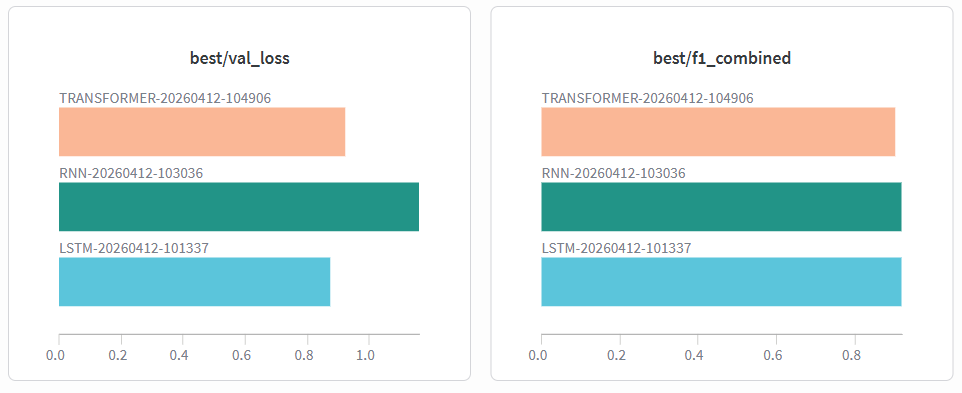
\includegraphics[width=\linewidth]{../images/wandb/wandb_best_metrics.png}
\caption{So sánh \texttt{best/val\_loss} và \texttt{best/f1\_combined} giữa 3 mô hình trên Weights \& Biases.}
\label{fig:wandb_best}
\end{figure}

\begin{figure}[H]
\centering
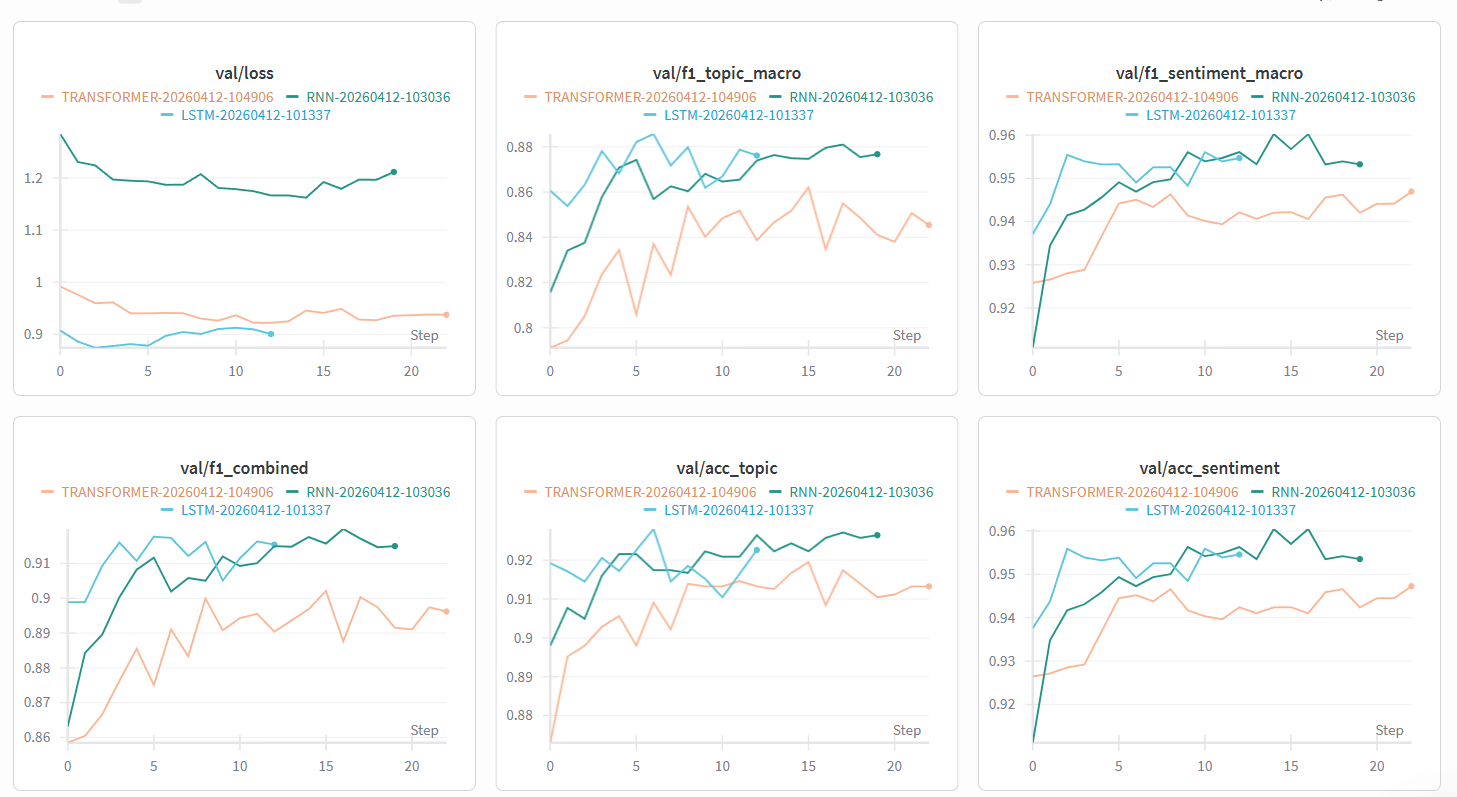
\includegraphics[width=\linewidth]{../images/wandb/wandb_learning_curves.png}
\caption{Diễn biến theo epoch của \texttt{val/loss}, \texttt{val/f1\_macro}, \texttt{val/f1\_combined} và \texttt{val/acc} trên Weights \& Biases.}
\label{fig:wandb_curves}
\end{figure}

Từ hai biểu đồ W\&B có thể rút ra các nhận xét chính:
\begin{itemize}
    \item \textbf{BiGRU cho quỹ đạo học ổn định và đều:} Đường \texttt{val/f1\_combined} tăng đều và duy trì ở mức cao ở giai đoạn cuối, đồng thời \texttt{val/acc\_topic} và \texttt{val/acc\_sentiment} ít dao động.
    \item \textbf{BiLSTM có \texttt{val/loss} thấp nhưng không vượt BiGRU ở chỉ số đa nhiệm:} Mặc dù đạt \texttt{val/loss} thấp hơn Transformer, \texttt{val/f1\_combined} của BiLSTM không nhỉnh hơn BiGRU do dữ liệu Topic bị mất cân bằng lớp.
    \item \textbf{Transformer hội tụ chậm và dao động ở Topic Macro-F1:} Đường \texttt{val/f1\_topic\_macro} của Transformer thấp hơn và dao động mạnh hơn hai mô hình hồi quy, cho thấy kiến trúc tự chú ý huấn luyện từ đầu khó nắm bắt các lớp thiểu số (\texttt{training\_program}, \texttt{facility}) trên tập dữ liệu cỡ trung bình.
    \item \textbf{Early Stopping phát huy hiệu quả:} Các đường metric đi vào vùng bão hòa (plateau) từ giữa đến cuối quá trình train; việc dừng sớm giúp tránh overfitting và tiết kiệm thời gian huấn luyện.
\end{itemize}

\subsection{Phân tích lỗi qua Ma trận nhầm lẫn}

\begin{figure}[H]
\centering
\begin{subfigure}[b]{0.495\linewidth}
    \centering
    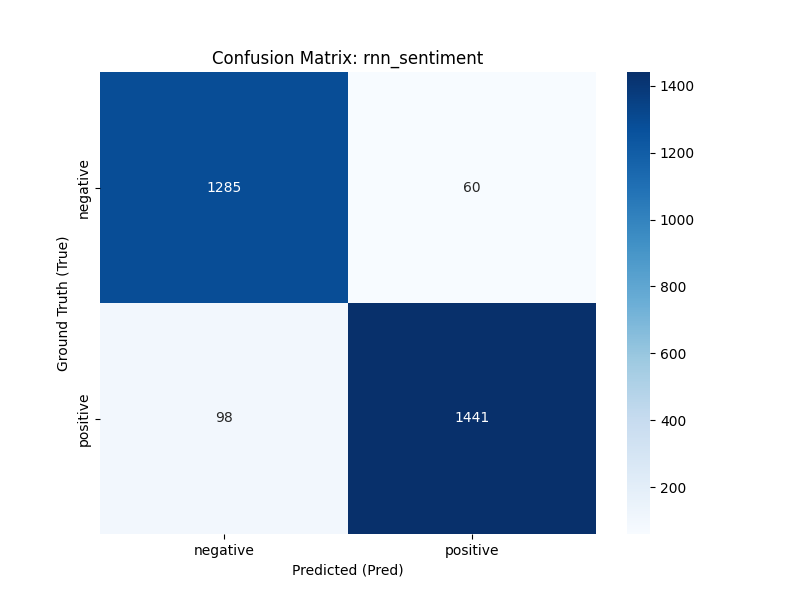
\includegraphics[width=\linewidth]{../images/rnn/rnn_sentiment_confusion_matrix.png}
    \caption{BidirRNN (BiGRU)}
\end{subfigure}
\hfill
\begin{subfigure}[b]{0.495\linewidth}
    \centering
    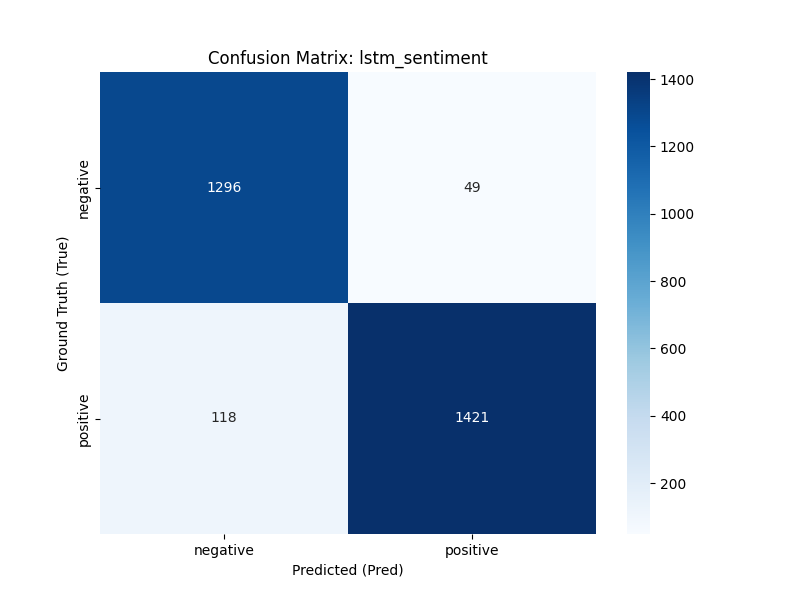
\includegraphics[width=\linewidth]{../images/lstm/lstm_sentiment_confusion_matrix.png}
    \caption{BidirLSTM}
\end{subfigure}
\\[0.6em]
\begin{subfigure}[b]{0.62\linewidth}
    \centering
    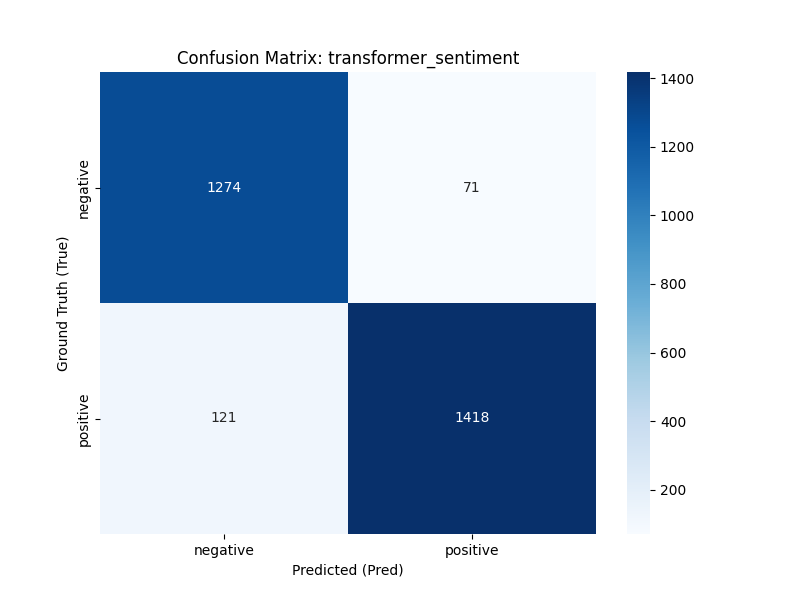
\includegraphics[width=\linewidth]{../images/transformer/transformer_sentiment_confusion_matrix.png}
    \caption{MultiTaskTransformer}
\end{subfigure}
\caption{Ma trận nhầm lẫn tác vụ Sentiment trên tập Test ($N = 2{,}884$).}
\label{fig:cm_sent}
\end{figure}

Trên tác vụ \textbf{Sentiment} (Hình~\ref{fig:cm_sent}), cả 3 mô hình đều đạt recall cao ở lớp \texttt{negative} ($0.95$--$0.97$); BiGRU chỉ nhầm 41 mẫu \texttt{negative} (3.0\%, so với 49 ở BiLSTM và 71 ở Transformer). Lỗi chủ yếu là các câu \texttt{positive} bị dự đoán nhầm thành \texttt{negative} (117--121 mẫu), thường gặp ở các phản hồi góp ý tích cực nhưng có chứa từ phủ định.

\begin{figure}[H]
\centering
\begin{subfigure}[b]{0.495\linewidth}
    \centering
    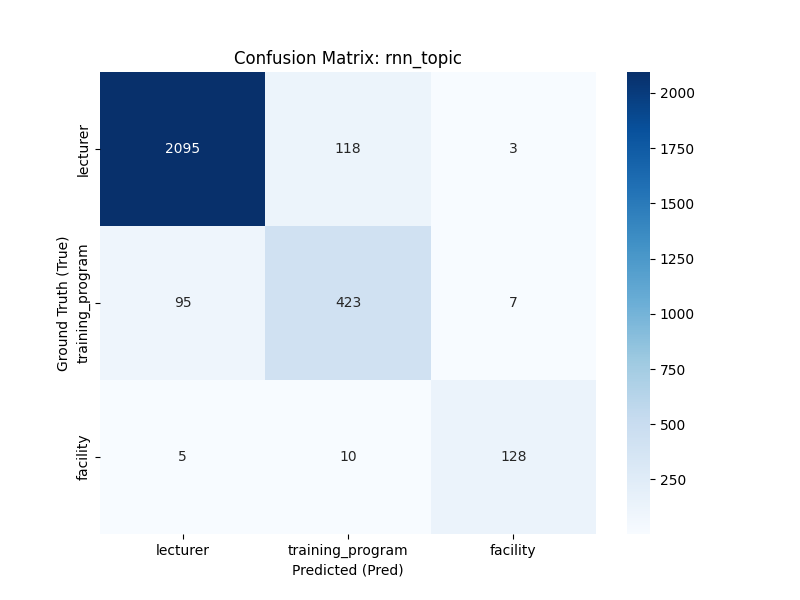
\includegraphics[width=\linewidth]{../images/rnn/rnn_topic_confusion_matrix.png}
    \caption{BidirRNN (BiGRU)}
\end{subfigure}
\hfill
\begin{subfigure}[b]{0.495\linewidth}
    \centering
    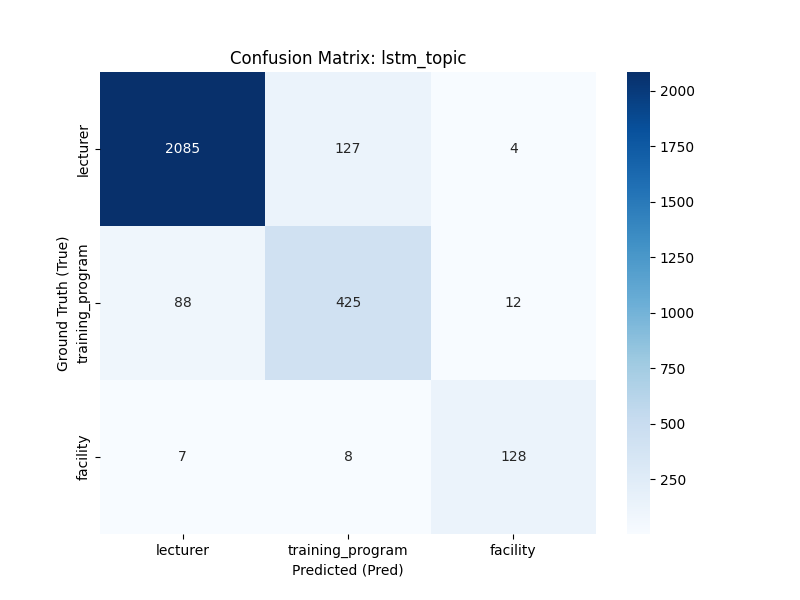
\includegraphics[width=\linewidth]{../images/lstm/lstm_topic_confusion_matrix.png}
    \caption{BidirLSTM}
\end{subfigure}
\\[0.6em]
\begin{subfigure}[b]{0.62\linewidth}
    \centering
    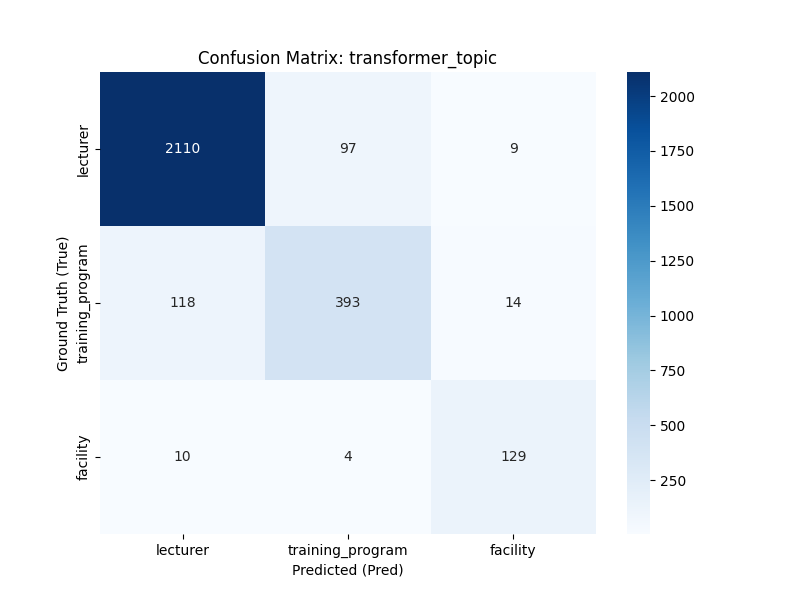
\includegraphics[width=\linewidth]{../images/transformer/transformer_topic_confusion_matrix.png}
    \caption{MultiTaskTransformer}
\end{subfigure}
\caption{Ma trận nhầm lẫn tác vụ Topic trên tập Test ($N = 2{,}884$).}
\label{fig:cm_topic}
\end{figure}

Trên tác vụ \textbf{Topic} (Hình~\ref{fig:cm_topic}):
\begin{itemize}
    \item \texttt{lecturer} đạt F1 \textbf{0.95} ở cả ba mô hình nhờ chiếm 76.8\% số mẫu.
    \item \texttt{training\_program} là lớp khó nhất (F1 $0.77$--$0.78$), hay bị nhầm sang \texttt{lecturer} (97--118 mẫu) do nội dung góp ý môn học thường nhắc kèm giảng viên.
    \item \texttt{facility} dù chỉ chiếm 5.0\% vẫn đạt F1 \textbf{0.90} trên BiGRU nhờ từ vựng đặc thù ít chồng lấn.
\end{itemize}

% =======================================================================
% 5. KẾT LUẬN VÀ LIÊM CHÍNH HỌC THUẬT
% =======================================================================
\section{Kết luận và Liêm chính Học thuật}

\subsection{Kết luận và Hướng phát triển}
Nhóm đã hoàn thiện nghiên cứu và thực nghiệm học đa nhiệm cho bài toán phân loại cảm xúc và chủ đề phản hồi sinh viên với ba kiến trúc \texttt{BidirLSTM}, \texttt{BidirRNN (BiGRU)} và \texttt{MultiTaskTransformer}. Kết quả đối chiếu công bằng với trọng số loss $(1.0, 1.0)$ cho thấy \texttt{BidirRNN (BiGRU)} đạt hiệu năng cao nhất (Avg F1 \textbf{0.915}) với kích thước mô hình gọn nhẹ nhất (1.95 MB). Hướng phát triển tiếp theo gồm: (1) áp dụng mô hình ngôn ngữ tiền huấn luyện tiếng Việt như \textit{PhoBERT} hoặc \textit{ViDeBERTa} để cải thiện ngữ cảnh giữa \texttt{training\_program} và \texttt{lecturer}, và (2) thử nghiệm hàm mất mát có trọng số lớp hoặc \textit{Focal Loss} nhằm cải thiện độ phủ ở các lớp thiểu số.

\subsection{Liên kết Dự án}
Mã nguồn đầy đủ, kết quả thực nghiệm và nhật ký huấn luyện của nhóm được công khai tại:
\begin{itemize}
    \item \textbf{GitHub Repository:} \url{https://github.com/HeroKeyboardUT/MultitaskLearning-P4AIDS}
    \item \textbf{Weights \& Biases Dashboard:} \href{https://wandb.ai/thienhao164/student-feedback?nw=nwuserthienhao164}{W\&B Dashboard -- Student Feedback} (\url{https://wandb.ai/thienhao164/student-feedback})
\end{itemize}

\subsection{Tuyên bố Liêm chính Học thuật}
Nhóm cam kết tuân thủ quy định liêm chính học thuật của môn học:
\begin{itemize}
    \item \textbf{Công cụ AI đã sử dụng:} Sử dụng trợ lý AI hỗ trợ rà soát thí nghiệm, dựng sơ đồ kiến trúc và định dạng tài liệu LaTeX.
    \item \textbf{Phần nhóm tự thực hiện và kiểm chứng:} Nhóm trực tiếp thiết kế phương pháp, chạy thực nghiệm thực tế trên tập dữ liệu, kiểm chứng toàn bộ số liệu và phân tích lỗi giữa các mô hình.
\end{itemize}

\end{document}
